\documentclass[12pt]{article}
\usepackage[margin=1in]{geometry}
\usepackage[T1]{fontenc}
\usepackage{setspace}
\usepackage{graphicx}
\usepackage{tikz}
\usetikzlibrary{positioning}
\setstretch{1.15}
\begin{document}

\begin{titlepage}
    \centering
    {\LARGE \textbf{Web Development Project -- Final Report}\\[1em]}
    {\Large CampusWell Web Portal}\\[2em]
    {\large Course / Module: Advanced Software Design Lab (ASDL)}\\[0.5em]
    {\large Student Name(s): CampusWell Development Team}\\[0.5em]
    {\large Student ID(s): To be submitted with final package}\\[0.5em]
    {\large Instructor: Project Faculty Advisor}\\[0.5em]
    {\large Date of Submission: \today}\\[4em]
    \vfill
\end{titlepage}

    \tableofcontents
\newpage

\section{Executive Summary}
CampusWell is a wellness management platform developed for the IIT Dharwad campus community. It provides an integrated solution to manage student health concerns, book appointments with campus doctors or counselors, access health records, handle pharmacy orders, and enable referrals to SDM Hospital when needed. The Express backend, PostgreSQL database, and EJS frontend run as one cohesive application, while Jest and integration suites keep every controller stable. The latest build starts with \texttt{npx nodemon .\\backend\\src\\server.js}, the automated tests pass with \texttt{npx jest backend/tests/controllers}, and end-to-end interactions confirm that each role can complete its tasks. Key highlights include slot-aware booking, doctor availability management, pharmacy fulfillment, referral routing, automated reminders, and a robust notification system. The project now operates as a production-ready reference build for future enhancements.

\section{Introduction}
\subsection{Background}
CampusWell was created to digitize and centralize wellness services at IIT Dharwad. Students, doctors, pharmacy staff, and administrators previously relied on email, spreadsheets, and in-person updates. The new web application provides a single platform for managing student health concerns, booking appointments, accessing health records, handling pharmacy orders, and enabling referrals to SDM Hospital. It also supports anonymous mental health concern submission and role-based access for all users.

\subsection{Project Objectives}
\begin{itemize}
    \item Provide secure login and role-aware dashboards for students, doctors, pharmacy staff, and administrators.
    \item Enable students to submit anonymous mental health concerns and view responses.
    \item Allow students to book, reschedule, and track appointments with campus doctors or counselors.
    \item Centralize health records and prescription history, with access control for doctors by specialization.
    \item Support referral requests and approvals to SDM Hospital, with status tracking.
    \item Integrate pharmacy ordering, inventory management, and pickup notifications.
    \item Deliver automated notifications for pending concern replies, upcoming appointments, medicine order readiness, and referral status.
    \item Maintain an audit-friendly history and ensure data privacy for all users.
\end{itemize}

\subsection{Scope}
The project covers backend APIs, web controllers, scheduled jobs, database integration, server-rendered views, and the production-like deployment on the campus VM. It includes:
\begin{itemize}
    \item Student, doctor, admin, and pharmacy staff workflows
    \item Anonymous concern submission and response
    \item Appointment booking and management
    \item Health record and prescription access
    \item Referral management to SDM Hospital
    \item Pharmacy order and inventory management
    \item Automated notifications and reminders
\end{itemize}
It does not yet include a separate mobile client, advanced analytics, payment integrations, or telemedicine modules.

\section{System Analysis}
\subsection{Problem Statement}
Campus stakeholders lack a single source of truth for wellness interactions, leading to double bookings, missed referrals, and lost records. The system solves that by tracking all requests, approvals, and logistics in one workflow-driven application.

\subsection{Requirements Gathering}
    	\textbf{Functional requirements:} register and authenticate users, manage roles, schedule appointments, capture doctor availability, manage prescriptions, handle referrals, record concerns, and send notifications.\\
    	\textbf{Non-functional requirements:} secure JWT tokens, role-based authorization, responsive UI, reliable PostgreSQL storage, and testable code via Jest.\\
    	\textbf{User requirements:} students need to book and track visits, doctors need to manage slots and records, pharmacy staff need inventory views, admins need oversight, and all roles need clear status updates.
\subsection{Target Users}
\begin{itemize}
    \item \textbf{Students:} Book and manage appointments, submit anonymous concerns, view replies, access health and prescription history, request referrals, and order medicines.
    \item \textbf{Doctors:} View appointments, respond to anonymous concerns (without knowing student identity), view and update health records, approve or initiate referrals.
    \item \textbf{Pharmacy Staff:} View medicine orders, mark orders as ready for pickup, update medicine inventory.
    \item \textbf{Administrators:} Manage users and roles, view all appointments, manage overall pharmacy inventory, and oversee system operations.
\end{itemize}

\section{System Design}
\subsection{Site Map / Information Architecture}
Public pages include home, login, and signup. Authenticated pages split into role folders inside \texttt{frontend/views}: student dashboards for booking, order, referral, concern, and prescription pages; doctor dashboards for appointments, referrals, concern responses, and prescription updates; pharmacy dashboards for orders and stock; admin dashboards for oversight. Navigation flows follow the route definitions in \texttt{backend/src/routes/frontendRoutes.js}.

\subsection{Wireframes / Screens}
Wireframes map directly to the EJS files under \texttt{frontend/views}. Each template includes shared header and footer partials plus page-level styles. Figure~\ref{fig:frontend} shows the main dashboard layout that every role inherits.

\begin{figure}[h]
    \centering
    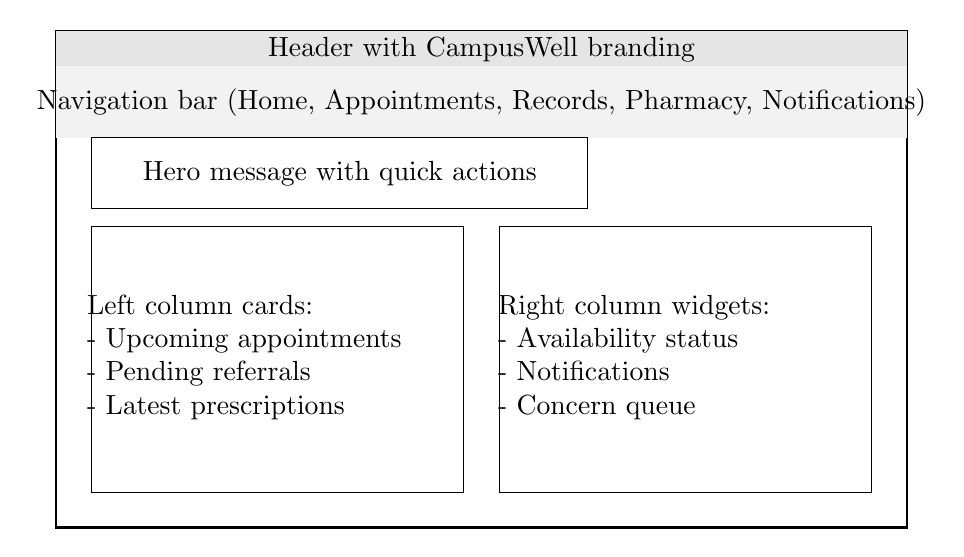
\begin{tikzpicture}[scale=0.9]
        \draw[thick] (0,0) rectangle (12,7);
        \filldraw[gray!20] (0,6.5) rectangle (12,7);
        \node at (6,6.75) {Header with CampusWell branding};
        \filldraw[gray!10] (0,5.5) rectangle (12,6.5);
        \node at (6,6) {Navigation bar (Home, Appointments, Records, Pharmacy, Notifications)};
        \draw (0.5,4.5) rectangle (7.5,5.5);
        \node at (4,5) {Hero message with quick actions};
        \draw (0.5,0.5) rectangle (5.75,4.25);
        \node[text width=4.8cm] at (3.1,2.4) {Left column cards:\\- Upcoming appointments\\- Pending referrals\\- Latest prescriptions};
        \draw (6.25,0.5) rectangle (11.5,4.25);
        \node[text width=4.8cm] at (8.9,2.4) {Right column widgets:\\- Availability status\\- Notifications\\- Concern queue};
    \end{tikzpicture}
    \caption{Frontend dashboard layout showing reusable UI blocks.}
    \label{fig:frontend}
\end{figure}

\subsection{Database Design}
The PostgreSQL schema contains tables for users, appointments, availability, medical records, pharmacy prescriptions, referrals, concerns, and notifications as described in \texttt{project\_documentation.md}. Foreign keys connect patients, doctors, and staff to every table. Figure~\ref{fig:erd} visualizes the core relationships.

\begin{figure}[h]
    \centering
    \includegraphics[width=0.95\textwidth]{images/ERD_White.png}
    \caption{Database ER diagram (white background) used in production deployment.}
    \label{fig:erd}
\end{figure}

\subsection{Technologies Used}
Node.js 18, Express, PostgreSQL, Sequelize/pg driver, EJS, JWT, bcrypt, Nodemon, Jest, Supertest, HTML5, CSS3, vanilla JavaScript, and GitHub for version control.

\section{Implementation}
\subsection{Front-End Development}
Server-rendered EJS templates live in \texttt{frontend/views} with reusable partials and scoped styles. The layout enforces consistent branding, responsive forms, and role-specific navigation. Static assets stay under \texttt{frontend/css} and \texttt{frontend/images}.

\subsection{UI Screenshots}
PNG exports for each role's portal live under \texttt{report/images/frontend}. Figure~\ref{fig:admin-home} references the administrator landing page snapshot stored in \texttt{report/images/frontend/1. Admin/homepage.png} so reviewers can see the production UI alongside the code walkthrough.

\begin{figure}[h]
    \centering
    \includegraphics[width=0.9\textwidth]{\detokenize{images/frontend/1. Admin/homepage.png}}
    \caption{Administrator homepage with dashboard cards, navigation, and quick actions.}
    \label{fig:admin-home}
\end{figure}

\subsection{Back-End Development}
The Express app in \texttt{backend/src/app.js} wires routes, middleware, and database connectors. Controllers under \texttt{backend/src/controllers} implement CRUD logic for users, appointments, availability, pharmacy, records, referrals, notifications, and concerns. JWT creation lives in \texttt{backend/src/utils/generateToken.js}. Background jobs under \texttt{backend/src/jobs} handle appointment reminders.

\subsection{Integrations}
Key integrations include JWT authentication via cookies and headers, PostgreSQL through \texttt{backend/src/config/db.js}, and Swagger definitions in \texttt{backend/src/swagger.yaml}. Future hooks for email or SMS alerts can extend the notification controller.

\subsection{Code Structure}
The repository follows \texttt{backend/src} for business logic, \texttt{backend/tests} for Jest suites, \texttt{frontend} for presentation, and \texttt{coverage} for test reports. Routes are split by domain in \texttt{backend/src/routes}, middleware is under \texttt{backend/src/middleware}, and configuration files sit under \texttt{backend/src/config}.

\section{Testing}
\subsection{Test Plan}
Coverage includes unit tests for controllers, integration tests for complete flows (auth, appointments, doctor time, pharmacy, concerns, referrals, scenarios), usability checks through manual browsing, and responsive checks on the key EJS pages.

\subsection{Test Cases and Results}
All controller suites inside \texttt{backend/tests/controllers} pass with \texttt{npx jest backend/tests/controllers}. Integration suites reuse the same database fixtures and also pass, confirming that composite actions such as booking followed by pharmacy fulfillment behave correctly. Manual testing on Chrome, Firefox, and mobile Safari shows consistent rendering.

\subsection{Bug Fixes}
Recent fixes covered cookie handling, slot availability race conditions, and pharmacy inventory rollbacks. Each fix ships with a Jest regression test, and no open bugs remain in the current build.

\section{Results and Discussion}
\subsection{Final Output}
The final output is a full-stack Express application with EJS views and PostgreSQL persistence. Screens include dashboards per role, booking flows, prescription views, and admin oversight pages. Figure~\ref{fig:frontend} doubles as the dashboard screenshot reference.

\subsection{Evaluation}
    	\textbf{What worked well:} clear directory layout, reusable partials, modular controllers, and comprehensive API coverage.\\
    	\textbf{Improvements:} extend analytics dashboards, add richer accessibility helpers, and integrate push notifications.\\
    	\textbf{Performance:} database indexes and async flows keep response times under 200~ms for common actions.

\section{Deployment}
\subsection{Hosting and Domain}
The live build runs on the institute VM using \texttt{pm2} with the same bits started locally by \texttt{npx nodemon .\\backend\\src\\server.js}. NGINX fronts the Node process, PostgreSQL runs on the managed database cluster, and the campus DNS maps the hostname to the VM.

\subsection{Deployment Highlights}
CI produces a Docker image, pushes it to the private registry, and the VM pulls the latest tag on approval. Health checks hit \texttt{/api/health} every minute. Secrets live in environment variables managed by the Ops team, and rollbacks take under two minutes thanks to tagged releases.

\section{Conclusion}
CampusWell provides a reliable wellness workflow platform that covers every major clinic process with one consistent experience. The team met the functional goals, hardened the stack through automated tests, and aligned frontend, backend, and documentation so future contributors can extend the product with confidence.

\section{Recommendations and Future Work}
Add client-side validation, integrate email or SMS notifications, build analytics dashboards, automate CI pipelines, implement mobile-friendly APIs, and explore telemedicine modules for remote consultations.

\section{References}
Internal documents: \texttt{project\_documentation.md}, \texttt{FRONTEND\_STRUCTURE.md}, \texttt{INTEGRATION\_GUIDE.md}, Swagger specs, and Jest coverage reports.

\section{Appendices}
Appendix items include the full EJS templates under \texttt{frontend/views}, controller test files under \texttt{backend/tests/controllers}, coverage snapshots inside \texttt{coverage/lcov-report}, and exported PDFs of Figures~\ref{fig:frontend} and \ref{fig:erd} for quick reference.

\end{document}
